\section{ADC Resampler} \label{subsec:ADCResampler}
The ADC Resampler block is generating the 'acquire start' (trigger) inputs for the ADC control block. When 'acquire start' for the ADC control module is asserted, the ADC control will start a single conversion. The ADC resampler will generate $N$ amount of trigger pulses for the ADC control block, with $M$ frequency. The full code listing for this module can be found in appendix \refq{App:ResamplerCode}.

The amount of pulses generated, i.e. the sample size $N$, and the sample frequency $M$ along with a 'start' signal is set by a number registers in the internal memory that was described in section \refq{subsec:Memory}. The signals going into, or out of, the ADC resampler can be seen on figure \refq{fig:7_2_10_RESAMPLE_IO}.

\begin{figure}[H]
    \centering
    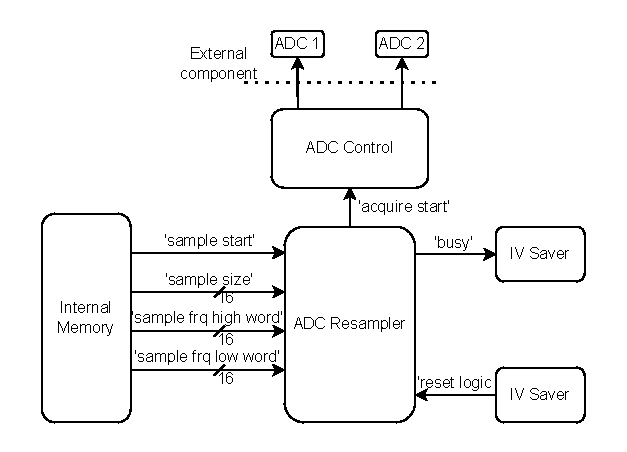
\includegraphics[clip, trim=0 0 0 0, width=0.9\textwidth]{Sections/7_SystemDesign/Figures/7_2_10_Resample_IO.pdf}
    \caption{A block diagram showing the I/O of the ADC resampler block. The ADC resampler also uses a \SIQ{200}{\mega\hertz} clock and a \SIQ{50}{\mega\hertz} clock, these are not shown on the block diagram.}
    \label{fig:7_2_10_RESAMPLE_IO}
\end{figure}

The module uses a Xilinx Direct Digital Synthesis (DDS) IP\cite{XILINXDDS} to generate the 'acquire start' pulses for the ADC control block. This is a black box component that was described briefly in section \refq{subsec:DAC_CONTROL} and it can be instantiated in an HDL project as a Vivado IP block for signal generation purposes. The output from the DDS module is a two's complement sine wave, but unlike the DAC control block, the ADC resampler block only requires the Numerically Controlled Oscillator portion of the DDS module in order to work, as it uses square waves and doesn't need to make use of the sine loop-up table in the DDS module. The ADC resampler block is getting a square wave from the DDS block by only using the MSb of the sine wave output. The DDS block uses a 48 bit control word, but only 32 bits are used as shown in the entity declaration in listing \refq{lst:7_2_10_ADCResampleEntity}.

\lstinputlisting[language=c ,style = c,firstnumber=1, linerange=37-49, caption={Code for DDS and DAC prescaler}, label={lst:7_2_10_ADCResampleEntity}]{Sections/7_SystemDesign/Code/adc_resampler.vhd}

The two signals, i\_sample\_frq\_low\_int\_mem\_reg and i\_sample\_frq\_high\_int\_mem\_reg, in lines 4 and 5 are concatenated with 0x0000 in order to form a 48 bit frequency control word for the DDS block. The DDS is using a \SIQ{50}{\mega\hertz} clock signal and this gives the DDS output a resolution of \SIQ{17.8}{\micro\hertz} as shown in equation \ref{eq:7_2_10_Fres}.

\begin{equation}\label{eq:7_2_10_Fres}
    f_{res} = \frac{f_{DDSCLK}}{2^N} = \frac{50e6}{2^{48}} = 1.776E-7
\end{equation}
This means the sample frequency of the ADC control block has a resolution of \SIQ{17.8}{\micro\hertz} as well.

The DDS block uses a phase accumulator and the size of the frequency control word affects the output jitter, a larger frequency control word reduces jitter as can be seen in the tests in appendix \refq{App:DDSJitter}. A 48 bit frequency control word is the largest that the DDS module can work with and is thus what is being used in this ADC resampler module.

The 'acq\_start' process in the ADC resampler runs when the 'r\_acq' flag is asserted in the internal memory as shown in code listying \refq{lst:7_2_10_ADC_RESAMPLER_ACQSTART}.

\lstinputlisting[language=C ,style = c,firstnumber=1, linerange=223-230, caption={VHDL code for starting the "resampler" process.}, label={lst:7_2_10_ADC_RESAMPLER_ACQSTART}]{Sections/7_SystemDesign/Code/adc_resampler.vhd}

A '1' on the 'r\_run\_sampler' signal starts the mealy meachine shown on figure \refq{fig:7_2_10_RESAMPLE_FSM}.

\begin{figure}[H]
    \centering
    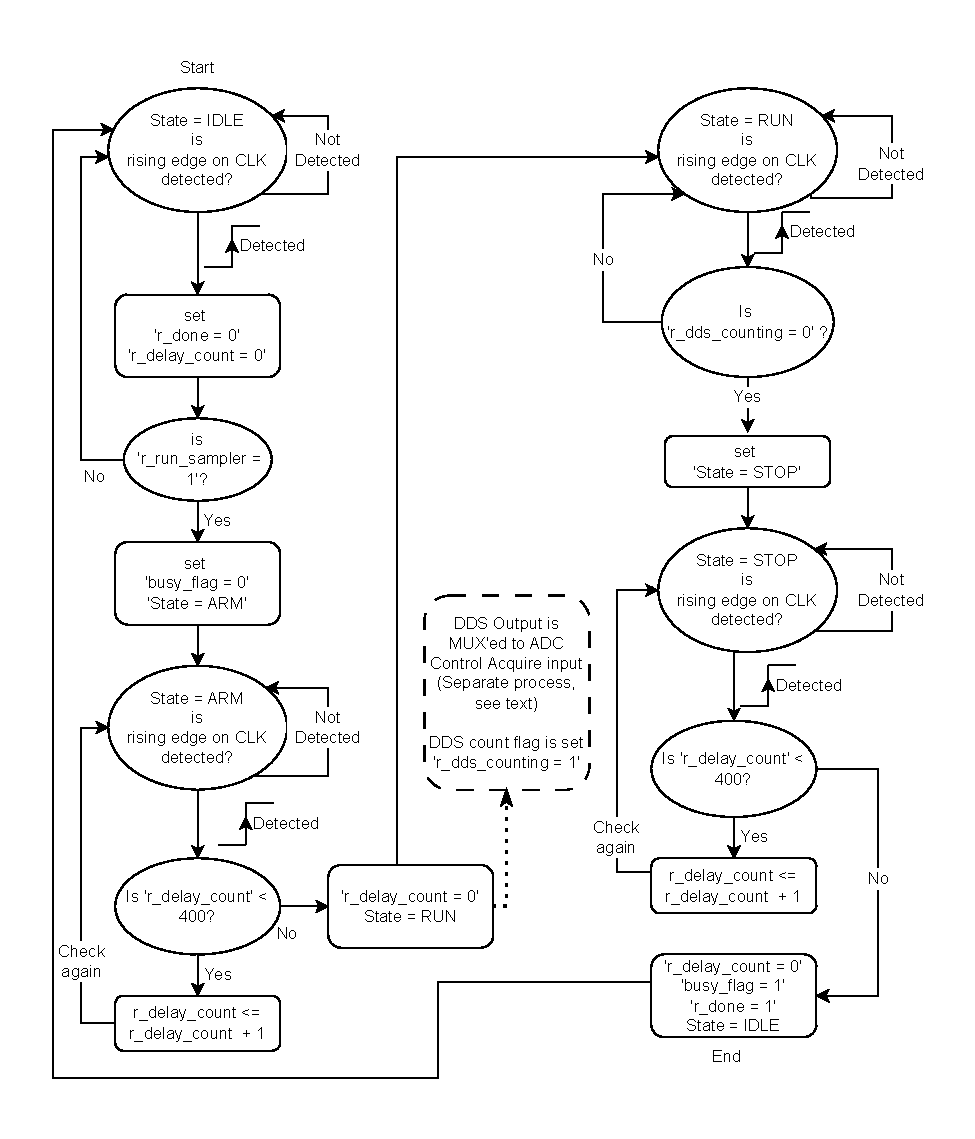
\includegraphics[clip, trim=0 0 0 0, width=0.9\textwidth]{Sections/7_SystemDesign/Figures/7_2_10_ADCResampler_FSM.pdf}
    \caption{The FSM controlling the ADC resampler process. The resampler starts in the IDLE state and if a rising edge on 'r\_acq' happens in the process in lising \refq{lst:7_2_10_ADC_RESAMPLER_ACQSTART} then it changes to the ARM state. The ARM state is a delay that is added to give the IV saver, external memory distribution and read/write blocks time to change from 'Read' to 'Write' mode, this is done by controlling the 'busy\_flag'. The busy flag is an ative low signal that is cleared when the state changes to ARM and set when state changes to IDLE. When the state changes to RUN this will signal another process to MUX the output of the DDS module to the ADC Control acquire trigger input. The process counts the amount of DDS CLKs until it reaches the desired amount of samples at which point it will set 'r\_dds\_counting = 0' and the state changes to STOP. The STOP state triggers another delay that is needed for timing purposes in the IV-saver, memory distribution and external memory logic path. After the delay has completed the state will change to the IDLE state and the FSM will wait for a new 'r\_acq' input.}
    \label{fig:7_2_10_RESAMPLE_FSM}
\end{figure}

The trigger signals for the ADC Control block are generated in the 'RUN' state as shown on the FSM diagram on figure \refq{fig:7_2_10_RESAMPLE_FSM}. The state transition to 'RUN' is what signals the process to start MUXing the DDS output to the ADC control input. The process is shown in listing \refq{lst:7_2_10_ADC_RESAMPLER_DDSCOUNT}. The 'r\_dds\_clk' signal is the output from the DDS and it's frequency depends on the frequency control word as described in the beginning of this section.

\lstinputlisting[language=C ,style = c,firstnumber=1, linerange=196-211, caption={VHDL Code for the DDS CLK MUX counting process}, label={lst:7_2_10_ADC_RESAMPLER_DDSCOUNT}]{Sections/7_SystemDesign/Code/adc_resampler.vhd}

The process in listing \refq{lst:7_2_10_ADC_RESAMPLER_DDSCOUNT} will, when asserted, MUX the output of the DDS to the ADC control block with the 'r\_dds\_mux\_enable' signal in lines 6 and 10. The process will count the amount of DDS CLK pulses generated and will keep asserting the 'r\_dds\_mux\_enable' signal until it has counted to an amount of CLKs equal to the 'r\_sample\_size' signal, which is set in the internal memory module. The ADC Control block will acquire an amount of samples from the ADCs that are equal to the amount of DDS CLKs generated.

The 'r\_dds\_mux\_enable' is an 'enable' signal for a special clock buffer \cite{BUGGCEClockBuffer} that is meant specifically for gating clock signals, like the DDS output. This is necessary because using "normal" gates can cause undesired behaviours and poor post-synthesis timing results.

